\documentclass[12pt]{article}
\usepackage{
  amsmath,
  booktabs,
  enumitem,
  geometry,
  graphicx,
  microtype,
  parskip,
}
\geometry{left=3cm, right=3cm, top=3cm, bottom=3cm}

% meta data
\newcommand{\chapter}{2.2}
\newcommand{\authorname}{Amo DelBello}
\newcommand{\classdescription}{MATH 1350-D2}
\newcommand{\classname}{Introduction to Statistics, Fall 2022}
\newcommand{\assignment}{\chapter\ Book Assignment}

\newcommand{\problem}[1]{\vspace{5ex}\section*{\chapter-#1}}
\newcommand{\thead}[1]{\textnormal{\textbf{#1}}}
\newcommand{\tvspace}{\vspace{.25cm}}

\title{\classdescription\ \\ \classname\ \\ $\ $ \\ \assignment}
\author{\authorname}
\date{\today}


\begin{document}
\maketitle

\problem{5}
The approximate number of quarters depicted in the three bars farthest to the left are $12 + 20 + 8 = 40$.


\problem{6}
The approximate value of the class width is $0.1$. The approximate value of the lower class limit is $5.5$ and the approximate value of the upper class limit is $5.6$


\problem{7}
The shape of the histogram would not change.


\problem{8}
A reasonable explanation is that the data set contains two different populations. This is mirrors the example of pennies being different weights based on their composition. Perhaps something similar happened to the composition of quarters.


\problem{10}
\begin{figure}[ht]
  \centering
  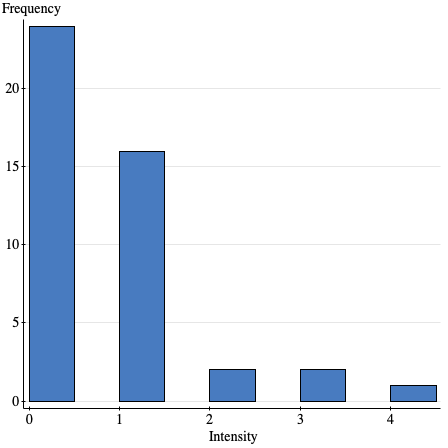
\includegraphics[width=10cm]{assets/tornado-frequency.png}
  \caption{Frequency distribution of tornado intensity}
\end{figure}

The histogram appears to be skewed to the right.

\problem{15}
\begin{figure}[h]
  \centering
  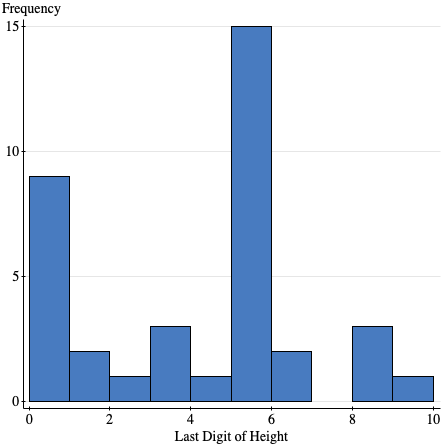
\includegraphics[width=10cm]{assets/last-digit-of-height.png}
  \caption{Frequency distribution of last digit of heights}
\end{figure}

The distribution of digits shows that most of the data was reported and not actually measured because most of the values are the round numbers of 0 and 5.

\end{document}
%%% Local Variables:
%%% mode: latex
%%% TeX-master: t
%%% End:
